\documentclass[]{report}
\usepackage{lmodern}
\usepackage{amssymb,amsmath}
\usepackage{ifxetex,ifluatex}
\usepackage{fixltx2e} % provides \textsubscript
\ifnum 0\ifxetex 1\fi\ifluatex 1\fi=0 % if pdftex
  \usepackage[T1]{fontenc}
  \usepackage[utf8]{inputenc}
\else % if luatex or xelatex
  \ifxetex
    \usepackage{mathspec}
  \else
    \usepackage{fontspec}
  \fi
  \defaultfontfeatures{Ligatures=TeX,Scale=MatchLowercase}
\fi
% use upquote if available, for straight quotes in verbatim environments
\IfFileExists{upquote.sty}{\usepackage{upquote}}{}
% use microtype if available
\IfFileExists{microtype.sty}{%
\usepackage{microtype}
\UseMicrotypeSet[protrusion]{basicmath} % disable protrusion for tt fonts
}{}
\usepackage[margin=1in]{geometry}
\usepackage{hyperref}
\hypersetup{unicode=true,
            pdfborder={0 0 0},
            breaklinks=true}
\urlstyle{same}  % don't use monospace font for urls
\usepackage{color}
\usepackage{fancyvrb}
\newcommand{\VerbBar}{|}
\newcommand{\VERB}{\Verb[commandchars=\\\{\}]}
\DefineVerbatimEnvironment{Highlighting}{Verbatim}{commandchars=\\\{\}}
% Add ',fontsize=\small' for more characters per line
\usepackage{framed}
\definecolor{shadecolor}{RGB}{248,248,248}
\newenvironment{Shaded}{\begin{snugshade}}{\end{snugshade}}
\newcommand{\KeywordTok}[1]{\textcolor[rgb]{0.13,0.29,0.53}{\textbf{#1}}}
\newcommand{\DataTypeTok}[1]{\textcolor[rgb]{0.13,0.29,0.53}{#1}}
\newcommand{\DecValTok}[1]{\textcolor[rgb]{0.00,0.00,0.81}{#1}}
\newcommand{\BaseNTok}[1]{\textcolor[rgb]{0.00,0.00,0.81}{#1}}
\newcommand{\FloatTok}[1]{\textcolor[rgb]{0.00,0.00,0.81}{#1}}
\newcommand{\ConstantTok}[1]{\textcolor[rgb]{0.00,0.00,0.00}{#1}}
\newcommand{\CharTok}[1]{\textcolor[rgb]{0.31,0.60,0.02}{#1}}
\newcommand{\SpecialCharTok}[1]{\textcolor[rgb]{0.00,0.00,0.00}{#1}}
\newcommand{\StringTok}[1]{\textcolor[rgb]{0.31,0.60,0.02}{#1}}
\newcommand{\VerbatimStringTok}[1]{\textcolor[rgb]{0.31,0.60,0.02}{#1}}
\newcommand{\SpecialStringTok}[1]{\textcolor[rgb]{0.31,0.60,0.02}{#1}}
\newcommand{\ImportTok}[1]{#1}
\newcommand{\CommentTok}[1]{\textcolor[rgb]{0.56,0.35,0.01}{\textit{#1}}}
\newcommand{\DocumentationTok}[1]{\textcolor[rgb]{0.56,0.35,0.01}{\textbf{\textit{#1}}}}
\newcommand{\AnnotationTok}[1]{\textcolor[rgb]{0.56,0.35,0.01}{\textbf{\textit{#1}}}}
\newcommand{\CommentVarTok}[1]{\textcolor[rgb]{0.56,0.35,0.01}{\textbf{\textit{#1}}}}
\newcommand{\OtherTok}[1]{\textcolor[rgb]{0.56,0.35,0.01}{#1}}
\newcommand{\FunctionTok}[1]{\textcolor[rgb]{0.00,0.00,0.00}{#1}}
\newcommand{\VariableTok}[1]{\textcolor[rgb]{0.00,0.00,0.00}{#1}}
\newcommand{\ControlFlowTok}[1]{\textcolor[rgb]{0.13,0.29,0.53}{\textbf{#1}}}
\newcommand{\OperatorTok}[1]{\textcolor[rgb]{0.81,0.36,0.00}{\textbf{#1}}}
\newcommand{\BuiltInTok}[1]{#1}
\newcommand{\ExtensionTok}[1]{#1}
\newcommand{\PreprocessorTok}[1]{\textcolor[rgb]{0.56,0.35,0.01}{\textit{#1}}}
\newcommand{\AttributeTok}[1]{\textcolor[rgb]{0.77,0.63,0.00}{#1}}
\newcommand{\RegionMarkerTok}[1]{#1}
\newcommand{\InformationTok}[1]{\textcolor[rgb]{0.56,0.35,0.01}{\textbf{\textit{#1}}}}
\newcommand{\WarningTok}[1]{\textcolor[rgb]{0.56,0.35,0.01}{\textbf{\textit{#1}}}}
\newcommand{\AlertTok}[1]{\textcolor[rgb]{0.94,0.16,0.16}{#1}}
\newcommand{\ErrorTok}[1]{\textcolor[rgb]{0.64,0.00,0.00}{\textbf{#1}}}
\newcommand{\NormalTok}[1]{#1}
\usepackage{graphicx,grffile}
\makeatletter
\def\maxwidth{\ifdim\Gin@nat@width>\linewidth\linewidth\else\Gin@nat@width\fi}
\def\maxheight{\ifdim\Gin@nat@height>\textheight\textheight\else\Gin@nat@height\fi}
\makeatother
% Scale images if necessary, so that they will not overflow the page
% margins by default, and it is still possible to overwrite the defaults
% using explicit options in \includegraphics[width, height, ...]{}
\setkeys{Gin}{width=\maxwidth,height=\maxheight,keepaspectratio}
\IfFileExists{parskip.sty}{%
\usepackage{parskip}
}{% else
\setlength{\parindent}{0pt}
\setlength{\parskip}{6pt plus 2pt minus 1pt}
}
\setlength{\emergencystretch}{3em}  % prevent overfull lines
\providecommand{\tightlist}{%
  \setlength{\itemsep}{0pt}\setlength{\parskip}{0pt}}
\setcounter{secnumdepth}{5}
% Redefines (sub)paragraphs to behave more like sections
\ifx\paragraph\undefined\else
\let\oldparagraph\paragraph
\renewcommand{\paragraph}[1]{\oldparagraph{#1}\mbox{}}
\fi
\ifx\subparagraph\undefined\else
\let\oldsubparagraph\subparagraph
\renewcommand{\subparagraph}[1]{\oldsubparagraph{#1}\mbox{}}
\fi

%%% Use protect on footnotes to avoid problems with footnotes in titles
\let\rmarkdownfootnote\footnote%
\def\footnote{\protect\rmarkdownfootnote}

%%% Change title format to be more compact
\usepackage{titling}

% Create subtitle command for use in maketitle
\newcommand{\subtitle}[1]{
  \posttitle{
    \begin{center}\large#1\end{center}
    }
}

\setlength{\droptitle}{-2em}

  \title{}
    \pretitle{\vspace{\droptitle}}
  \posttitle{}
    \author{}
    \preauthor{}\postauthor{}
    \date{}
    \predate{}\postdate{}
  
\usepackage{mdframed}
\usepackage[utf8]{inputenc}
\usepackage[francais]{babel} % use french to compile pdf
\usepackage{geometry} % use to modify the margins
\geometry{hmargin = 4cm, vmargin = 3cm}
\usepackage{hyperref}
\usepackage{cite}
\usepackage{tocloft}
\newcommand*\rfrac[2]{{}^{#1}\!/_{#2}}

\begin{document}

\begin{centering}

\begin{figure}


\includegraphics[width=3.5cm, height=6cm]{../image/technique-logo.jpg} 

\includegraphics[width=5cm,height=7cm]{../image/UMONS-logo.jpg}
\includegraphics[width=1.8cm,height=3.5cm]{../image/ECONUM-logo.pdf}

\end{figure}

\textcolor{white}{.}

\vspace{2.5 cm}

\Huge

{\bf Rapport de stage partiel}

\vspace{1 cm}

\huge 
{\bf Mise en place d'une application web surveillant la croissance des coraux en mésocosmes.}
%Développement d'une application Shiny
\vspace{1 cm}

\Large

Jordan Benrezkallah

\vspace{2 cm}

\normalsize
Maître de stage : Philippe Grosjean

Encadrant de stage : Guyliann Engels

Promoteur : Aline Leonet et David Coornaert


\vspace{3.5 cm}

\normalsize
HEH - Campus technique -
Bloc 3 du cursus Bachelier en Biotechnique

Année académique 2018-2019

\end {centering}

\tableofcontents

\chapter{Présentation de
l'entreprise}\label{presentation-de-lentreprise}

Mon stage de fin d'études, se déroule dans à l'université de l'UMons
dans le service d'Écologie Numérique des Milieux Aquatiques (abrégé en
EcoNum) du département de Biologie.

L'Université de Mons (UMONS), est une université francophone implantée
en Belgique, dans la province du Hainaut. Elle est constituée de 2
écoles et de 7 facultés, dont la faculté des Sciences.

Le Département de biologie de la faculté des Sciences est impliqué dans
la formation des étudiants et dans la recherche.

Le département de biologie de la faculté des Sciences comprend 5
services dont le service d'Écologie Numérique des Milieux Aquatiques. Ce
dernier étudie les écosystèmes aquatiques complexes, tels les
communautés planctoniques et les récifs coralliens, face aux changements
de leur environnement.

Le Service développe également des outils en science des données, y
compris dans le domaine du data mining, des big data, et de la recherche
reproductible. Il participe à des études sur les logiciels Open Source.

Le laboratoire d'EcoNum est situé sur le campus de la plaine de Nimy (A)
(voir figure 1.1) dans le pentagone (1) (voir figure 1.2).

\begin{figure}
\centering
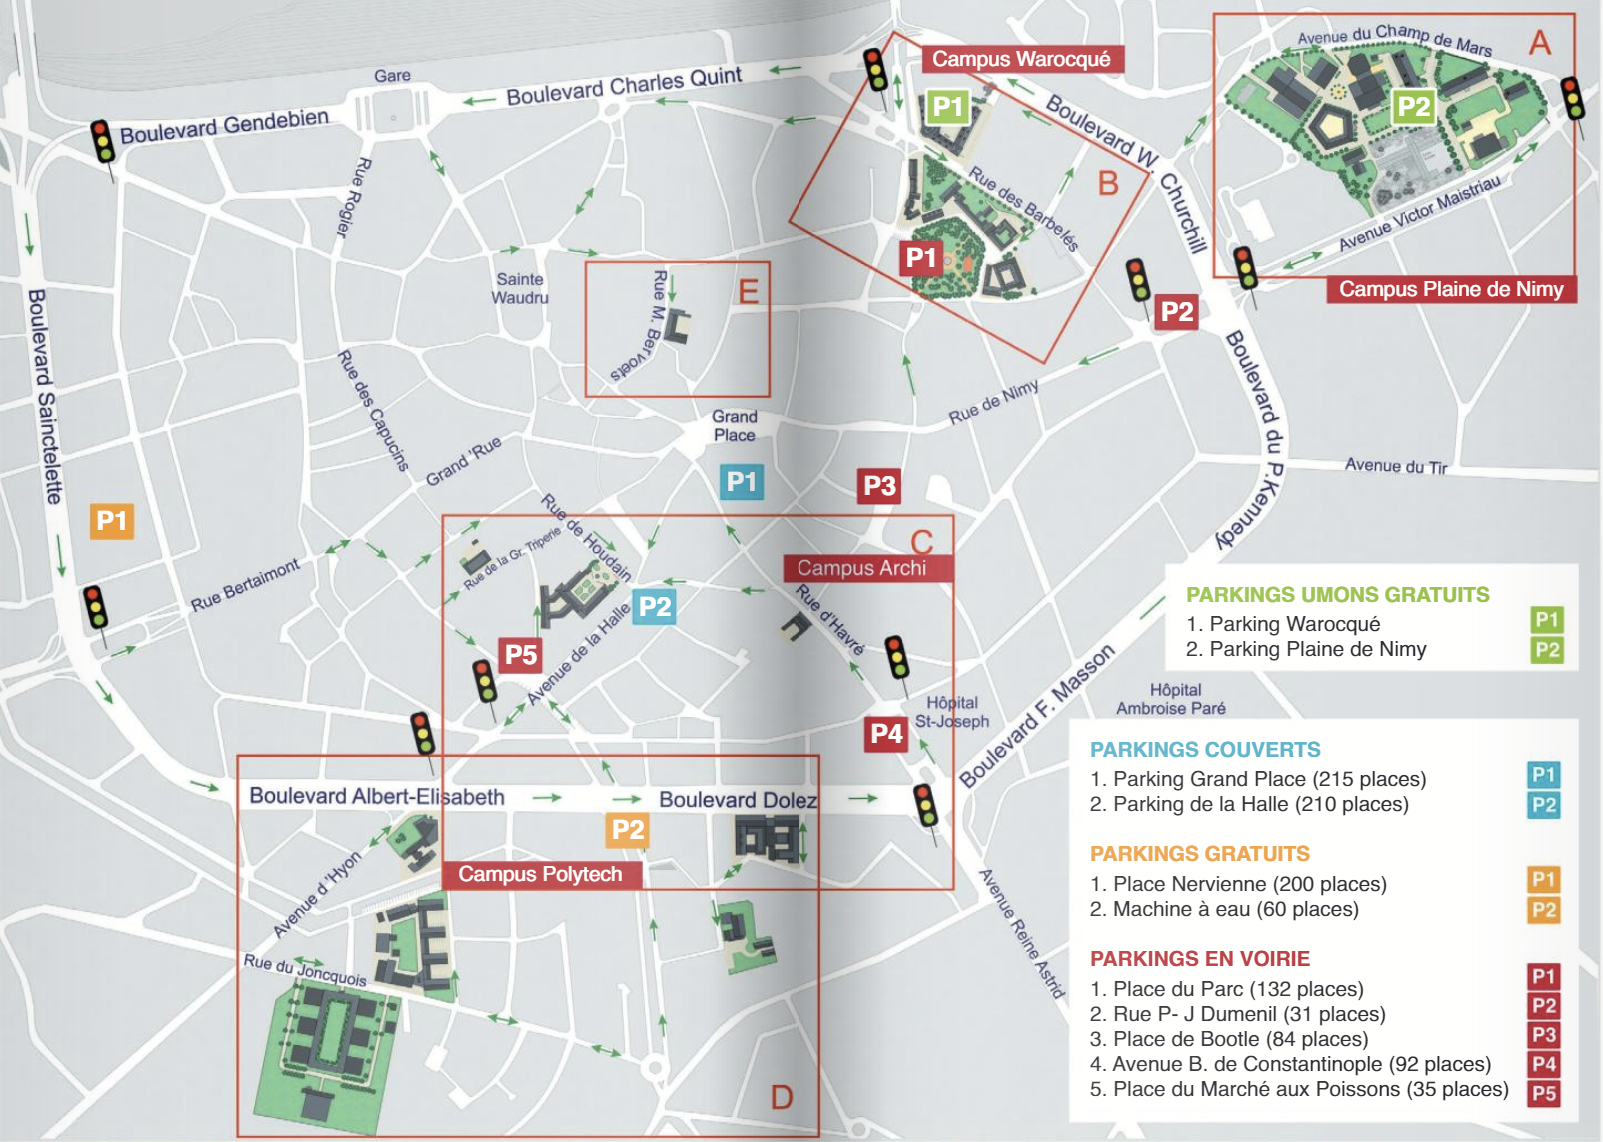
\includegraphics{../image/plan-campus.png}
\caption{Carte de la ville de Mons}
\end{figure}

\begin{figure}
\centering
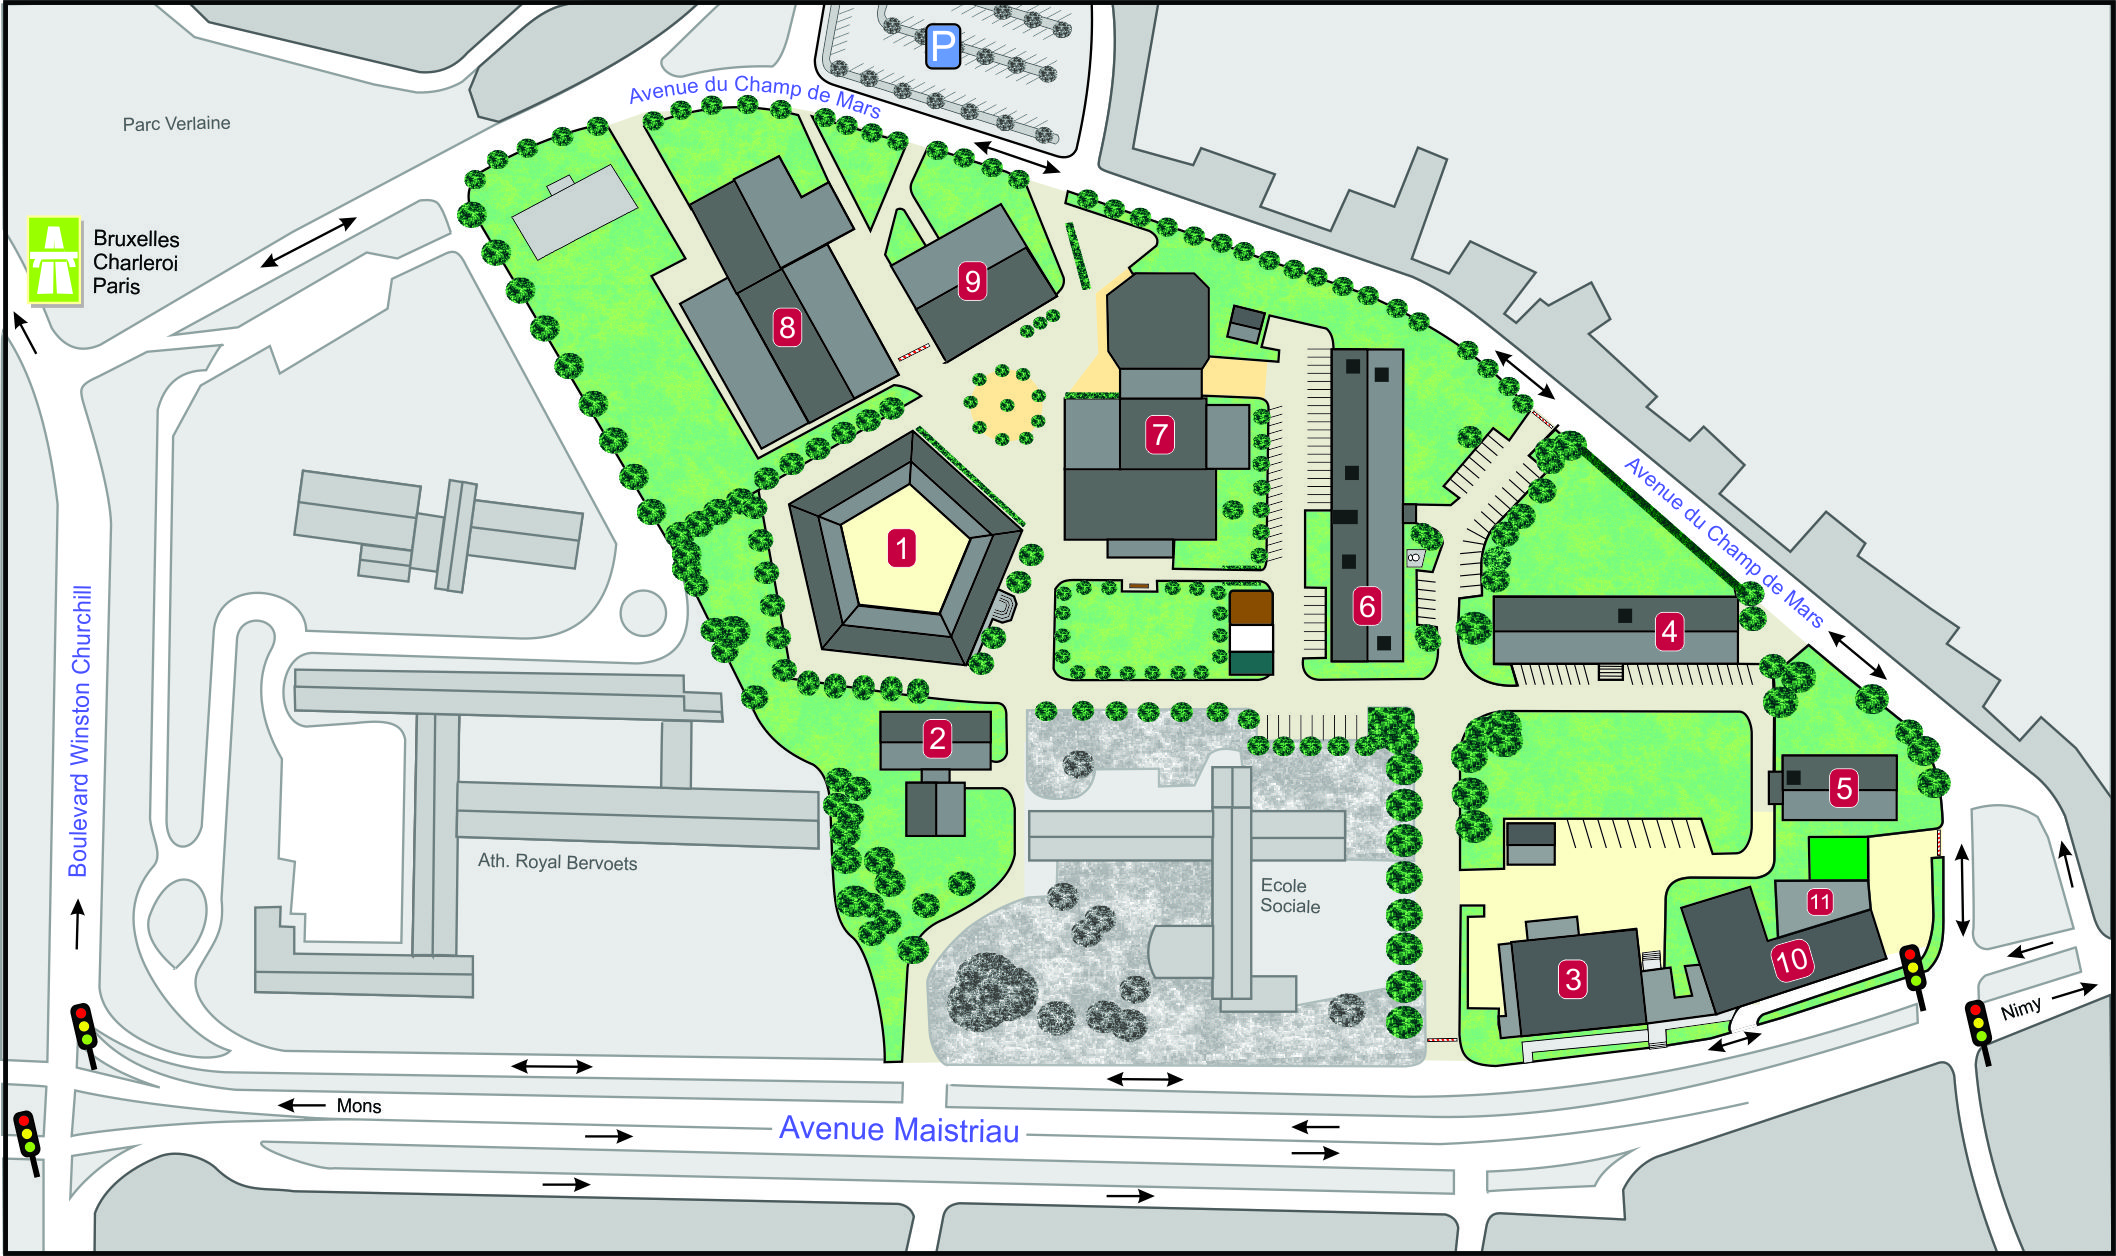
\includegraphics{../image/plaine-Nimy.jpg}
\caption{Carte du campus de la plaine de Nimy}
\end{figure}

\chapter{Présentation de l'équipe}\label{presentation-de-lequipe}

\section{Philippe Grosjean}\label{philippe-grosjean}

\begin{figure}[h!]

\includegraphics[width=4cm]{../image/Grosjean2.jpg}
\caption{Monsieur Philippe Grosjean, chef du service d'EcoNum.}
\end{figure}

Mon maître de stage est Monsieur Philippe Grosjean. Il mène plusieurs
projets de recherches sur l'identification automatique du plancton par
des algorithmes de \emph{machine learning}, sur l'écophysiologie des
scléractiniaires et sur le développement de logiciel pour l'écologie.

Il enseigne également la science des données biologiques, l'écologie
marine, l'écophysiologie et l'océanographie générale aux étudiants en
biologie.

Il développe des outils Open Source comme la \emph{SciViews Box}, qui
est une machine virtuelle contenant une suite de logiciel pré-configuré
pour l'utilisation de ses étudiants et des chercheurs.

Il encadre 1 doctorant et 2 étudiants en masters.

\section{Guyliann Engels}\label{guyliann-engels}

\begin{figure}[h!]

\includegraphics[width=4cm]{../image/Guyliann.jpg}
\caption{Guyliann Engels, doctorant encadrant le stage.}
\end{figure}

Guyliann Engels est chercheur et assistant au sein du service. Il
effectue sa thèse sur l'écophysiologie du corail, où il utilise un
mésocosme pour étudier les stress des coraux engendrés par la
modification de leurs nutriments essentiels (composés azotés et
phosphorés). Il utilise fréquemment les outils de statistiques R et
RStudio (avec R Markdown, R Notebook).

Il encadre mon travail.

\section{Antoine Batigny}\label{antoine-batigny}

\begin{figure}[h!]
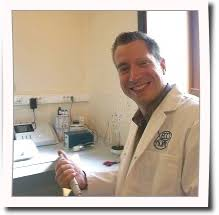
\includegraphics[width=4cm]{../image/antoine2.jpg}
\caption{Technicien du service d'EcoNum.}
\end{figure}

Antoine Batigny est le technicien du service. Il s'occupe principalement
de gérer les mésocosmes.

\section{Rémy Dugauquier}\label{remy-dugauquier}

\begin{figure}[h!]
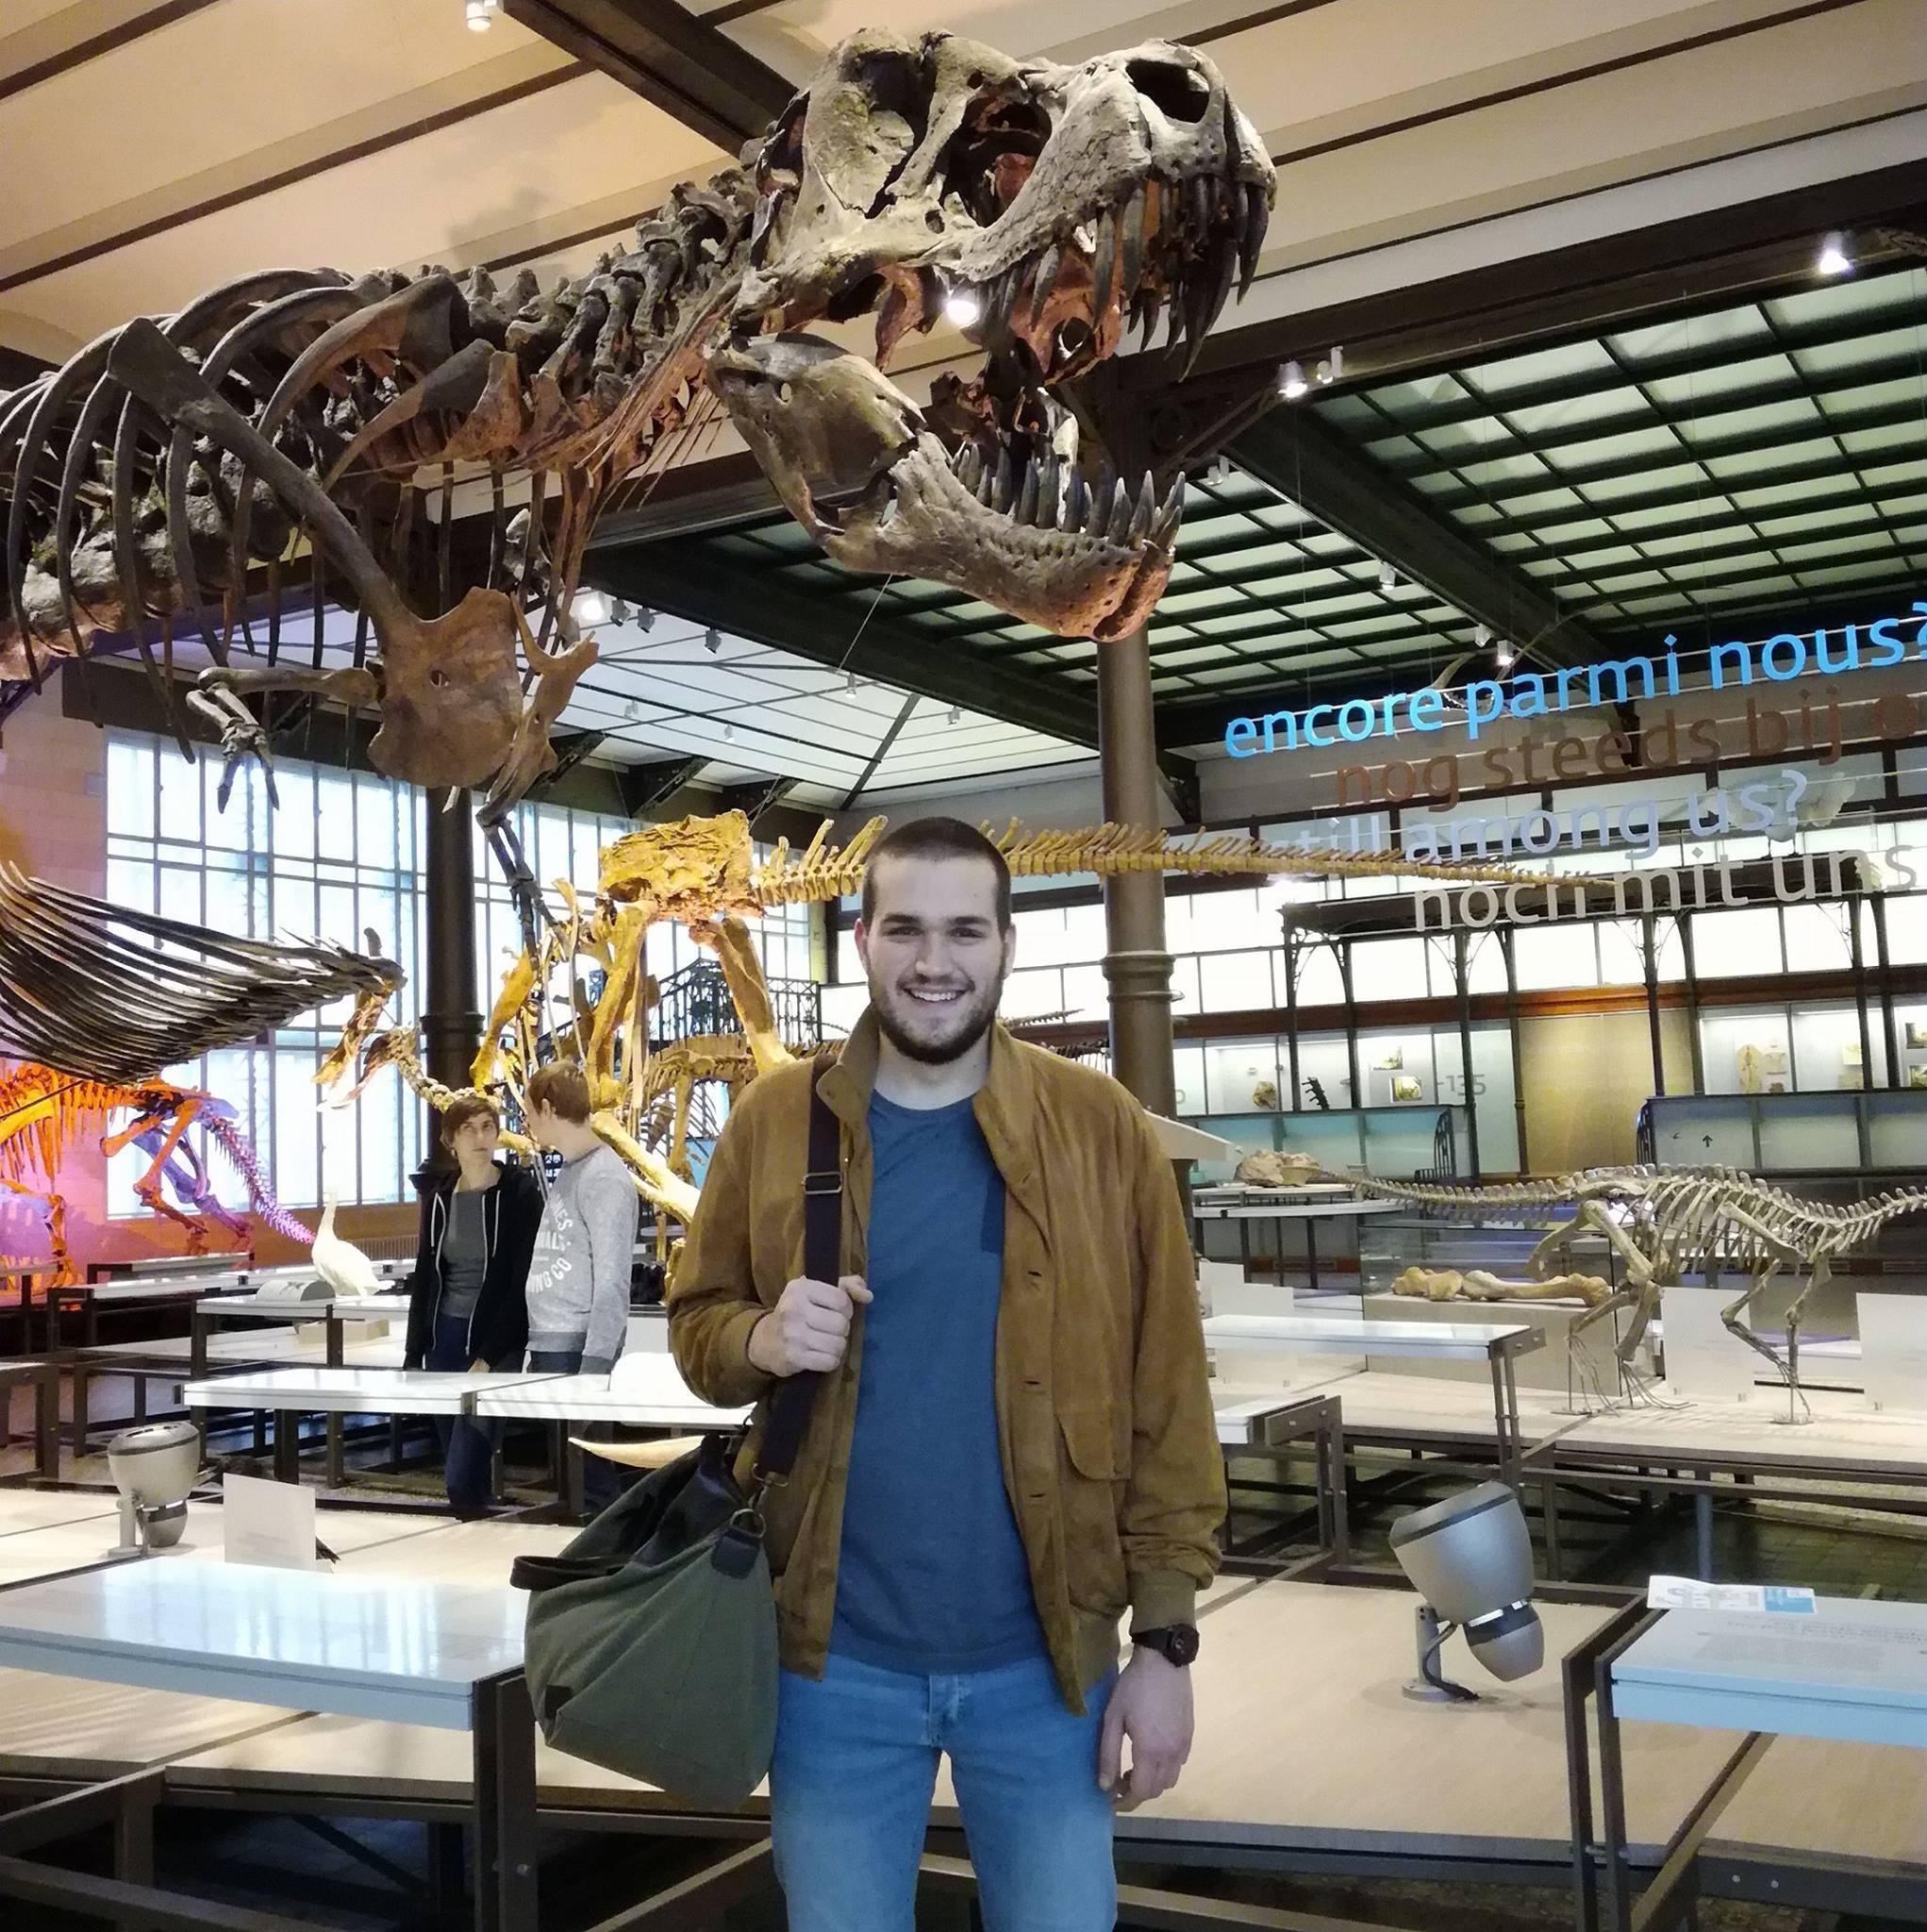
\includegraphics[width=4cm]{../image/remy.jpg}
\caption{Etudiant en master}
\end{figure}

Rémy Dugauquier est en dernière année du master en biologie des
organismes et écologie. Il réalise son T.F.E. sur l'écologie des
organismes planctoniques en baie de Calvi, France.

\section{Madeleine Gille}\label{madeleine-gille}

\begin{figure}[h!]

\includegraphics[width=4cm]{../image/madeleine.jpg}
\caption{Etudiante en master}
\end{figure}

Madeleine Gille est étudiante en dernière année du master en biologie
des organismes et écologie. Elle réalise son T.F.E. sur les effets d'un
stress salins (hyper et hyposalin) sur \emph{Seriatopora hystrix} (Dana,
1815).

\chapter{But}\label{but}

Le but du stage est de créer une application web via le package Shiny
dévelopé par RStudio sur R, qui suit l'évolution des coraux dans les
mésocosmes. Les coraux seront utilisés dans des expériences par le
laboratoire, il est donc nécessaire de visualiser leur croissance.
L'application doit pouvoir être utilisée facilement par d'autres
personnes à \emph{posteriori}, il faut donc l'automatiser et anticiper
les problèmes à venir.

Le stage se déroule en 2 parties, la première est une phase
d'apprentissage, la deuxième est la création de l'application et
l'implémentation d'outils pour le monitoring de la croissance des
coraux.

La phase d'apprentissage comprend :

\begin{itemize}
\tightlist
\item
  Apprentissage du langage de programmation R, de ses packages et de
  l'environnement RStudio.
\end{itemize}

La phase de création d'outils comprend :

\begin{itemize}
\item
  L'acquisition des données de croissance régulière des coraux.
\item
  La réalisation d'une application web Shiny, surveillant la croissance
  (monitoring) des coraux de l'espèce \emph{S. hystrix}.
\end{itemize}

\section{Outils monitorings}\label{outils-monitorings}

\subsection{Masse immergée et masse
squelettique}\label{masse-immergee-et-masse-squelettique}

Pour évaluer la croissance des boutures de coraux, on utilise la masse
squelettique. Pour l'obtenir sans détruire le corail, on mesure la masse
immergée du corail dans l'eau de mer avec une balance munie d'un
crochet. Cette méthodde de mesure est rapide et peu stressante pour les
organismes. Après avoir mesuré la température et la salinité on peut
convertir la masse immergée en masse squelettique à l'aide de la formule
ci-dessous mise au point par Jokiel \emph{et al} (1978) :

\begin{equation}
\large
  m_{squelettique} = \frac {m_{immerge}}{ \frac{1 - \rho_{eau}}{ \rho_{squelettique}}}
\end{equation}

\(\rho_{eau}\) est déterminé via l'équation d'état de l'eau de mer grâce
à la mesure de la salinité et de la température. Le
\(\rho_{squelettique}\) est la densité de l'aragonite(CaCO3) du
squelette du corail.

\subsection{Tableur}\label{tableur}

Les mesures effectuées sur les coraux et les paramètres de l'eau des
mésocosmes sont encodé dans un tableau de données.

Pour l'instant, j'utilise ma licence d'Excel d'office 365 fourni par la
HEH. Par la suite, j'aimerai utiliser un tableur en ligne afin que
n'importe qui, qui a besoin de remplir un tableau de donnée puisse le
faire depuis n'importe quelle machine connectée à internet.

Afin d'éviter au maximum des erreurs d'encodages, j'ai utilisé des
règles pour mettre en évidence les cases non remplies, formater le type
des cellules et mettre un dégradé de couleur suivant l'avancement des
données.

\begin{figure}[h!]
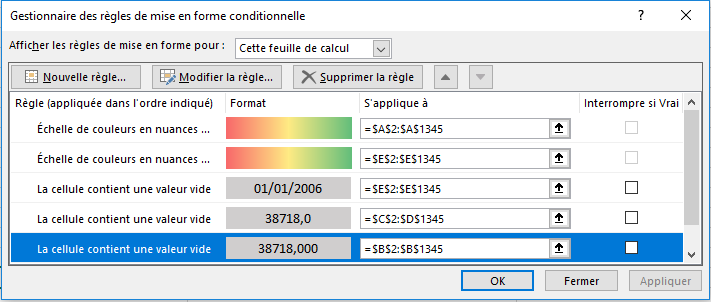
\includegraphics[]{../image/excel3.PNG}
\caption{Mise en forme conditionnelle d'Excel}
\end{figure}

Le tableau de donnée contient 7 colonnes :

\begin{itemize}
\item
  ID : corresponds à l'identifiant de la bouture.
\item
  weight : corresponds à la masse immergée de la bouture.
\item
  temp : corresponds à la température de l'eau de mer.
\item
  salinity : corresponds à la salinité de l'eau de mer
\item
  date : corresponds à la date et heure du relevé.
\item
  commentaire : donne quelques annotations.
\end{itemize}

\begin{figure}[h!]
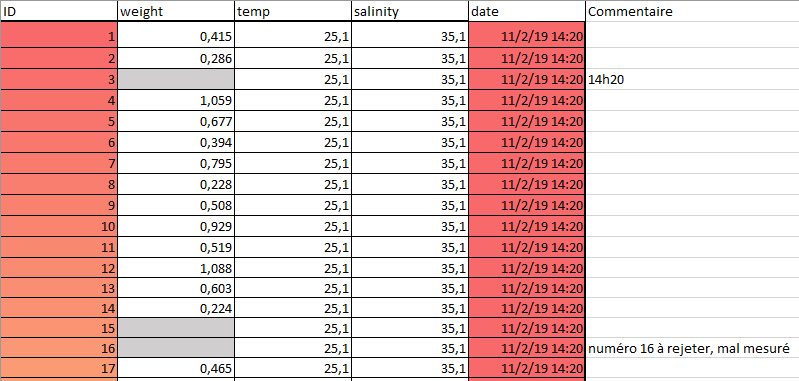
\includegraphics[]{../image/excel1.PNG}
\caption{Tableau de donnée}
\end{figure}

\subsection{Application Shiny}\label{application-shiny}

L'application est divisée en deux éléments, une partie ``ui'' (User
Interface), c'est la partie qui affiche les éléments graphiques de
l'interface Shiny à l'utilisateur, et une partie ``server'', qui
contient toutes les commandes R qui s'opère côté serveur.

Il est possible mettre l'intégralité du code dans un seul fichier app.R,
mais pour plus de clarté j'ai divisé mon script en deux fichiers ui.R et
server.R (voir page annexe).

Mon application présente 2 onglets, le premier créer un graphique
interactif.

\begin{figure}[h!]
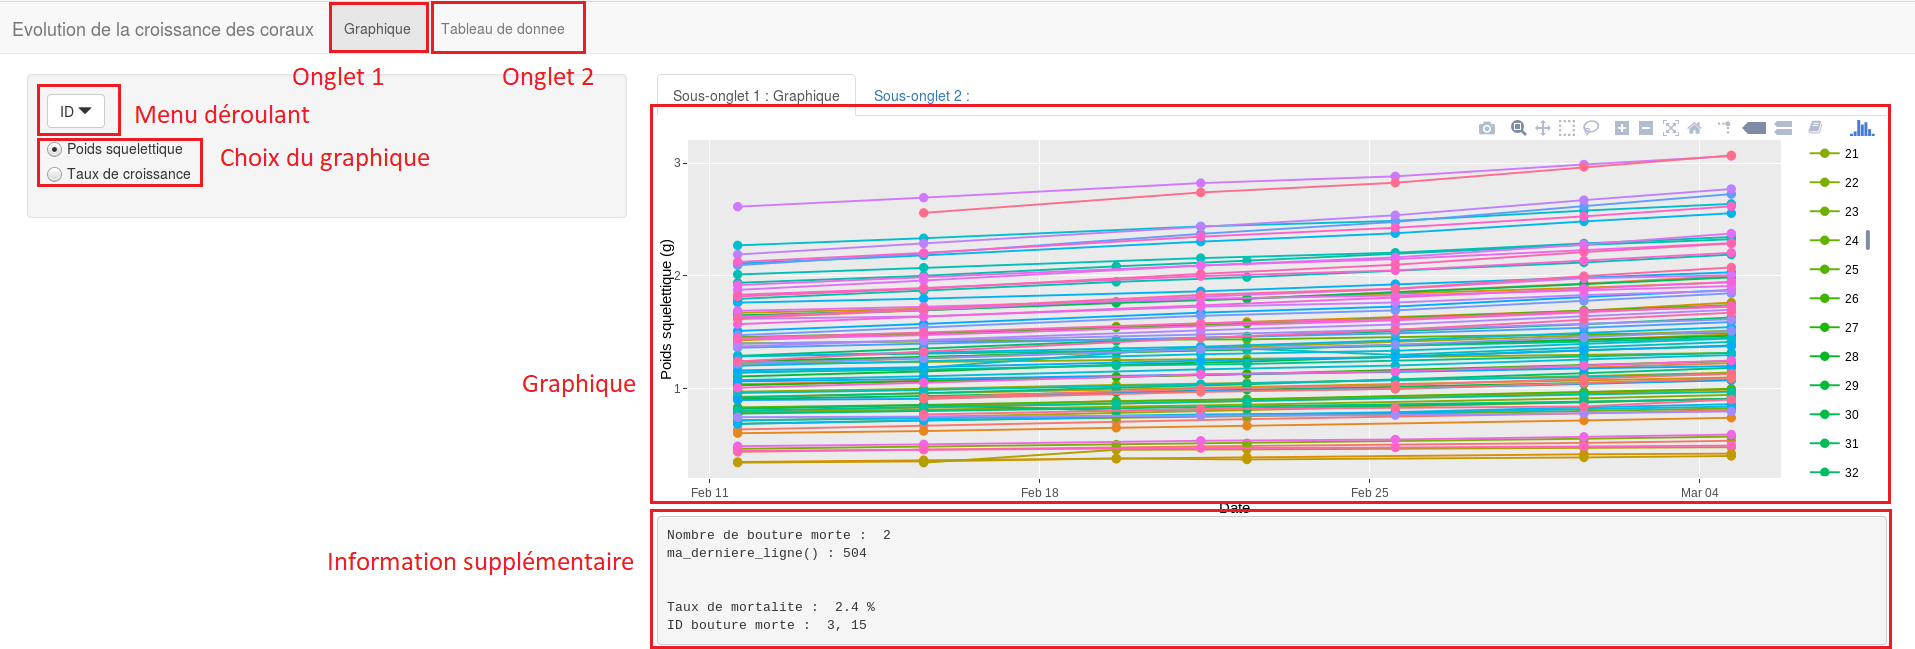
\includegraphics[]{../image/shiny1.PNG}
\caption{Application Shiny : légende}
\end{figure}

Par défaut, le graphique montre l'évolution de la masse squelettique en
fonction du temps.

\begin{figure}[h!]
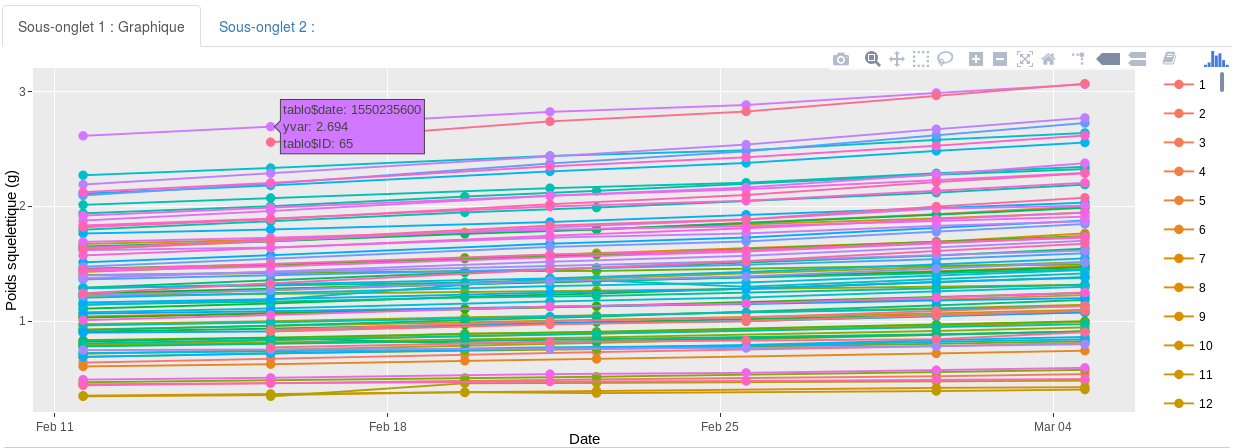
\includegraphics[]{../image/shiny2.PNG}
\caption{Application Shiny : masse squelettique}
\end{figure}

On peut sélectionner le taux de croissance en fonction du temps.

\begin{figure}[h!]
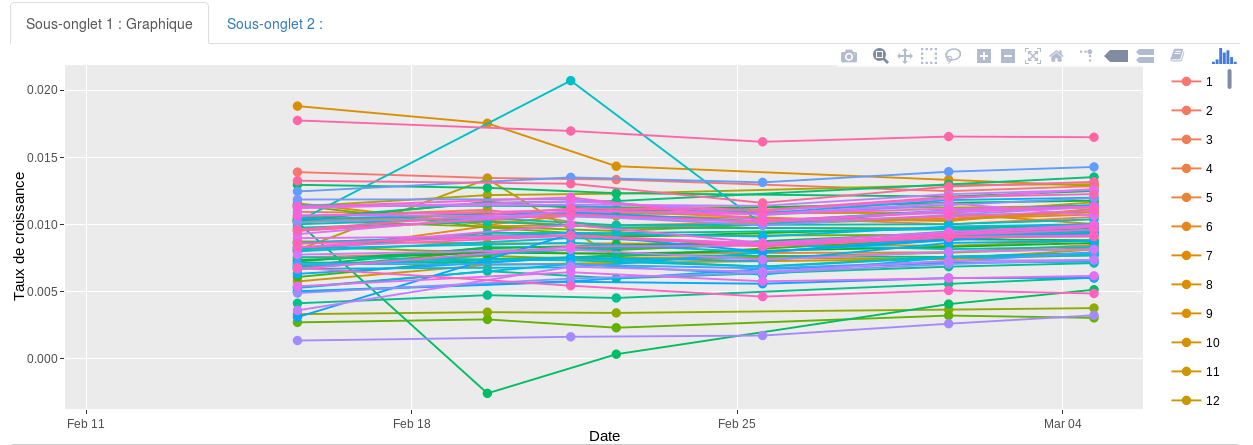
\includegraphics[]{../image/shiny3.PNG}
\caption{Application Shiny : taux de croissance}
\end{figure}

Il est possible de sélectionner les ID dans un menu déroulant ou de
directement cliquer à droite du graphique sur les ID triés par couleur.

Le menu déroulant permet de tout sélectionner ou de tout désélectionner.

\begin{figure}[h!]
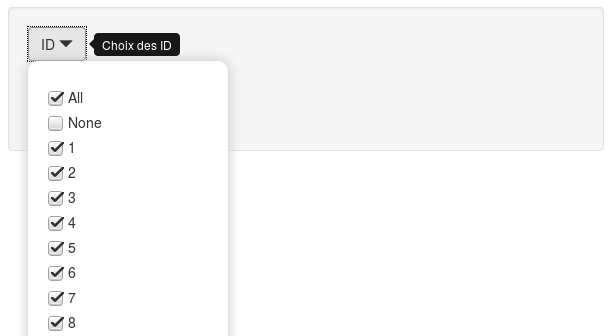
\includegraphics[]{../image/shiny4.PNG}
\caption{Application Shiny : menu déroulant}
\end{figure}

\begin{figure}[h!]
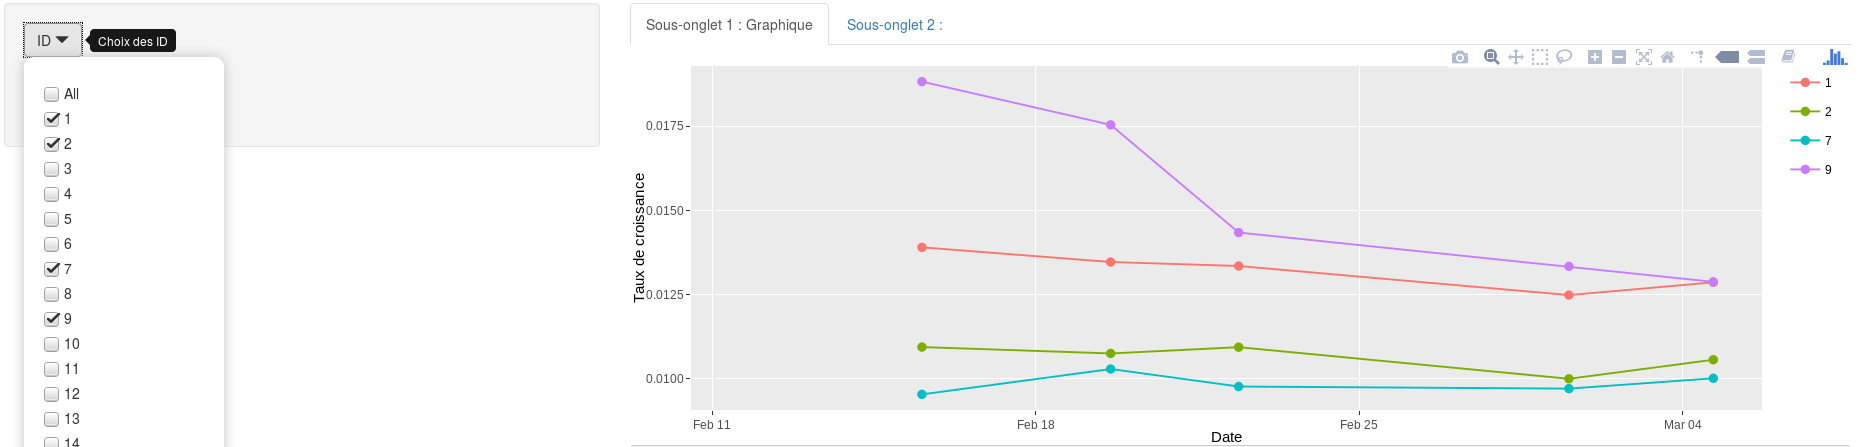
\includegraphics[]{../image/shiny5.PNG}
\caption{Application Shiny : affichage intéractif}
\end{figure}

En passant le curseur sur les points du graphique, on peut obtenir
quelques informations.

Sous le graphique, des informations supplémentaires : le nombre de
boutures mortes, leur ID et le taux de mortalité sont calculés.

\begin{figure}[h!]
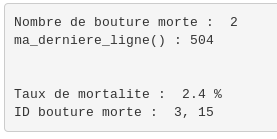
\includegraphics[]{../image/shiny7.PNG}
\caption{Application Shiny : informations supplémentaires}
\end{figure}

Le deuxième onglet contient le tableau de donnée où de nouvelles
colonnes ont été calculées, il y a l'ajout de la masse squelettique et
du ``ratio'' qui correspond au taux de croissance.

\begin{figure}[h!]
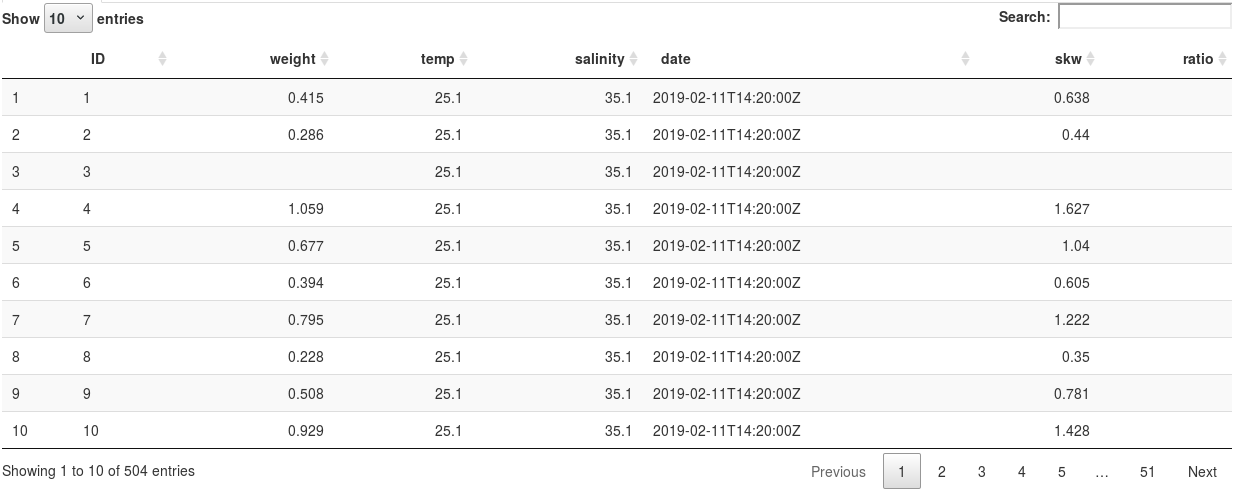
\includegraphics[]{../image/shiny8.PNG}
\caption{Application Shiny : tableau de donnée}
\end{figure}

\section{Outils utilisés}\label{outils-utilises}

Les outils utilisés sont :

\begin{itemize}
\item
  La machine virtuelle \emph{SciViews Box}, contenant un linux
  (Xubuntu), R, RStudio et les paquets nécessaires pré-installés.
\item
  Les langages de programmation : R.
\item
  Les paquets : Shiny, tidyverse, ggplot2, dyplyr, plotly, googlesheets,
  ect.
\end{itemize}

\section{Objectifs réalisés}\label{objectifs-realises}

Les objectifs réalisés sont :

\begin{itemize}
\item
  Bouturer les coraux et relever leurs masses immergées.
\item
  Créer un tableau Excel contenant les données nécessaires.
\item
  Créer un prototype d'application web à l'aide du paquet Shiny.
\end{itemize}

\section{Planning de travail}\label{planning-de-travail}

Les horaires de stages sont flexibles, on peut arriver entre 7 et 9
heure et il faut prester au moins 8 heures par jour.

\chapter{Communications
interpersonnelles}\label{communications-interpersonnelles}

\section{Difficultés rencontrées}\label{difficultes-rencontrees}

\subsection{R vs python}\label{r-vs-python}

La principale difficulté rencontrée au début est de passer de
l'apprentissage du langage de programmation \emph{python} à \emph{R}. Ce
sont tous les deux des langages de programmation interprétés.
\emph{python} a été créé pour faire de la programmation informatique
généraliste, il est utilisé dans de larges domaines par des
informaticiens. A l'inverse, R est dédié aux analyses statistiques,
plutôt utilisées par des spécialistes ou des scientifiques.

Dans le domaine du \emph{data scientist}, \emph{R} et \emph{python} sont
courament employé.

\subsection{Shiny communication entre ui.R et
server.R}\label{shiny-communication-entre-ui.r-et-server.r}

Les application web géré par shiny utilise deux fonctions communiquant
entre elles \textbf{ui} et le \textbf{server}

Le schéma de communication basique entre les deux scripts commence par
la déclaration d'une variable \emph{inputId = ma\_variable} dans ui.R.
Celui-ci est ensuite appelé dans server.R sous la forme
input\$ma\_variable, cette variable sera ensuite traitée dans un bloc de
code délimiter par des crochets.

Shiny utilise du Javascript pour dynamiser l'interface de l'utilisateur
sous une couche de code masqué, cette couche simplifie grandement le
travail avec R. Si on sort du cadre de l'utilisation prévu par Shiny, on
se heurte à de grands soucis de codage. Shiny restreint donc, la
communication entre les différents blocs de code. Dans certaines
situations cela complique le travail.

\subsection{Apport au sein de
l'entreprise}\label{apport-au-sein-de-lentreprise}

\ldots{}

\chapter{Annexe}\label{annexe}

\begin{Shaded}
\begin{Highlighting}[]
\KeywordTok{library}\NormalTok{(shiny)}
\KeywordTok{library}\NormalTok{(shinyWidgets)}
\KeywordTok{library}\NormalTok{(DT)}
\KeywordTok{library}\NormalTok{(plotly)}
\KeywordTok{library}\NormalTok{(shinythemes)}

\KeywordTok{shinyUI}\NormalTok{(}
  \KeywordTok{navbarPage}\NormalTok{(}
    \CommentTok{# theme = shinytheme("slate"),}
    \DataTypeTok{title =} \StringTok{"Evolution de la croissance des coraux"}\NormalTok{, }\CommentTok{# Titre onglet 1}
    \KeywordTok{tabPanel}\NormalTok{(}\StringTok{"Graphique"}\NormalTok{, }\CommentTok{# Onglet principal 1}
             \CommentTok{# Sidebar : volet de gauche - Input}
             \KeywordTok{sidebarPanel}\NormalTok{(}
               \KeywordTok{uiOutput}\NormalTok{(}\DataTypeTok{outputId =} \StringTok{"ID"}\NormalTok{),}\CommentTok{# Selection des ID a afficher}
               \KeywordTok{uiOutput}\NormalTok{(}\DataTypeTok{outputId =} \StringTok{"Ratio"}\NormalTok{)}
\NormalTok{             ),}

             \CommentTok{# mainPanel : Volet de droite - Output}
             \KeywordTok{mainPanel}\NormalTok{(}
               \KeywordTok{tabsetPanel}\NormalTok{( }\CommentTok{# Sous-onglet}
                 \KeywordTok{tabPanel}\NormalTok{(}\StringTok{"Sous-onglet 1 : Graphique"}\NormalTok{,}
                          \KeywordTok{plotlyOutput}\NormalTok{(}\DataTypeTok{outputId =} \StringTok{"monplot"}\NormalTok{),}
                          \CommentTok{#sortie console}
                          \KeywordTok{verbatimTextOutput}\NormalTok{(}\DataTypeTok{outputId =} \StringTok{"boutures_mortes"}\NormalTok{)),}
                 \KeywordTok{tabPanel}\NormalTok{(}\StringTok{"Sous-onglet 2 : "}\NormalTok{)}
\NormalTok{               )}
\NormalTok{             )}
\NormalTok{    ),}
    \KeywordTok{tabPanel}\NormalTok{(}\StringTok{"Tableau de donnee"}\NormalTok{, }\CommentTok{# Onglet principal 2}
             \CommentTok{# sidebar : volet de gauche - Input}
             \KeywordTok{sidebarPanel}\NormalTok{(}
\NormalTok{             ),}
             \CommentTok{# mainPanel : Volet de droite - Output}
             \KeywordTok{mainPanel}\NormalTok{(}
               \KeywordTok{tabsetPanel}\NormalTok{(}
                 \KeywordTok{tabPanel}\NormalTok{(}\StringTok{"Beau tablo"}\NormalTok{, DT}\OperatorTok{::}\KeywordTok{dataTableOutput}\NormalTok{(}\StringTok{"tableau"}\NormalTok{))}
\NormalTok{               )}
\NormalTok{             )}
\NormalTok{    )}
\NormalTok{  )}
\NormalTok{)}
\end{Highlighting}
\end{Shaded}

\begin{Shaded}
\begin{Highlighting}[]
\CommentTok{#                 |                                                            #}
\CommentTok{#                 |                                                            #}
\CommentTok{#                ,|.                                                           #}
\CommentTok{#               ,\textbackslash{}|/.                                                          #}
\CommentTok{#             ,' .V. `.                                                        #}
\CommentTok{#            / .     . \textbackslash{}                                                       #}
\CommentTok{#           /_`       '_\textbackslash{}                                                      #}
\CommentTok{#          ,' .:     ;, `.                                                     #}
\CommentTok{#          |@)|  . .  |(@|                                                     #}
\CommentTok{#     ,-._ `._';  .  :`_,' _,-.                                                #}
\CommentTok{#    '--  `-\textbackslash{} /,-===-.\textbackslash{} /-'  --`                                               #}
\CommentTok{#   (----  _|  ||___||  |_  ----)                                              #}
\CommentTok{#    `._,-'  \textbackslash{}  `-.-'  /  `-._,'                                               #}
\CommentTok{#             `-.___,-'                                                        #}

\NormalTok{################################__INFO__########################################}
\CommentTok{# Application Shiny}
\CommentTok{# creer un graphique et un tableau a partir d'un fichier .csv}
\CommentTok{# les valeurs manquantes "NA" sont detecter comme etant des boutures mortes.}
\CommentTok{#}
\CommentTok{# Pour utiliser correctement l'application,}
\CommentTok{# il est important de respecter la syntaxe des noms des colonnes qui sont :}
\CommentTok{# |     ID     |     weight     |     temp     |    salinity    |     date     |}
\CommentTok{#}
\CommentTok{# Le format de la date doit etre de type :}
\CommentTok{# dd/mm/yyyy}
\CommentTok{#}
\CommentTok{# Il est egalement necessaire de commenter les lignes :}
\CommentTok{#cp_tablo[81:84, 2] <- "oublie"}
\CommentTok{#cp_tablo[16, 2] <- "a rejeter"}
\CommentTok{#botablo[81:84, 2] <- "oublie"}
\CommentTok{#botablo[16, 2] <- "a rejeter"}
\CommentTok{#}
\CommentTok{# Ces lignes sont specifiques a mon jeux de donnees}
\NormalTok{################################################################################}
\CommentTok{#}
\CommentTok{# Titre  : Croissance des coraux}
\CommentTok{# Auteur : Jordan Benrezkallah}
\CommentTok{# Date debut : 04/03/2019}
\CommentTok{# Date fin : 06/05/2019}
\CommentTok{#}
\NormalTok{################################################################################}

\CommentTok{# Importation des librairies :}

\KeywordTok{library}\NormalTok{(shiny)}
\KeywordTok{library}\NormalTok{(ggplot2)}
\KeywordTok{library}\NormalTok{(lubridate)}
\KeywordTok{library}\NormalTok{(tidyverse)}
\KeywordTok{library}\NormalTok{(dplyr)}
\KeywordTok{library}\NormalTok{(plotly)}
\KeywordTok{library}\NormalTok{(googlesheets)}
\NormalTok{SciViews}\OperatorTok{::}\NormalTok{R}
\CommentTok{# library(scales)}

\CommentTok{# #Fonction de Raphael :}
\CommentTok{# source(file = "../R/fonctions.R")}
\CommentTok{# #Mes fonctions}
\CommentTok{# source(file = "../R/fonction.R")}


\CommentTok{# Importation de mes donnees (format csv)}
\CommentTok{#correction a faire : chemin relatif}
\CommentTok{#tablo <- gdata::read.xls("~/shared/Github/coral_growth001/data/raw/monBordel/tablo.xlsx")}

\NormalTok{tablo <-}\StringTok{ }\KeywordTok{read.table}\NormalTok{(}\StringTok{"~/shared/Github/coral_growth001/data/my_data/tablogs.csv"}\NormalTok{, }\DataTypeTok{header =} \OtherTok{TRUE}\NormalTok{, }\DataTypeTok{sep =} \StringTok{";"}\NormalTok{, }\DataTypeTok{dec =} \StringTok{","}\NormalTok{)}

\CommentTok{# GOOGLE SHEETS#}
\CommentTok{# tablo <- gs_title("tablo")}
\CommentTok{# tablo <- gs_read(tablo)}
\CommentTok{# tablo}

\CommentTok{# Determination du nombre de ligne de tableau a utiliser}
\CommentTok{# /!\textbackslash{} Baser sur la premiere valeur NA rencontre dans la colonne "temp" /!\textbackslash{}}
\CommentTok{# Fonction a ameliorer de facon a ne garder seulement les lignes completes (ID, weight, temp, salinity, date)}

\NormalTok{ma_derniere_ligne <-}\StringTok{ }\ControlFlowTok{function}\NormalTok{()\{}
\NormalTok{  a <-}\StringTok{ }\DecValTok{0}
  \ControlFlowTok{for}\NormalTok{ (i }\ControlFlowTok{in}\NormalTok{ tablo}\OperatorTok{$}\NormalTok{temp) \{}
    \ControlFlowTok{if}\NormalTok{ (}\OperatorTok{!}\KeywordTok{is.na}\NormalTok{(i)) \{}
\NormalTok{      a <-}\StringTok{ }\NormalTok{a }\OperatorTok{+}\StringTok{ }\DecValTok{1}
\NormalTok{    \}}
\NormalTok{  \}}
  \KeywordTok{return}\NormalTok{(a)}
\NormalTok{\}}

\CommentTok{# Extraction des 5 colonnes (id, weight,temp,salinity et date) jusqu'a la derniere}
\CommentTok{# ligne de la colonne "temp" du fichier .csv}
\NormalTok{tablo <-}\StringTok{ }\NormalTok{tablo[}\DecValTok{1}\OperatorTok{:}\KeywordTok{ma_derniere_ligne}\NormalTok{(), }\DecValTok{1}\OperatorTok{:}\DecValTok{5}\NormalTok{]}

\NormalTok{### Calcul du poids squelettique :}
\CommentTok{#a corriger : rho_aragonite}
\CommentTok{#P = Pression hydrostatique, elle vaut 0 a la surface}
\NormalTok{skeleton_weight <-}\StringTok{ }\ControlFlowTok{function}\NormalTok{(}\DataTypeTok{S =}\NormalTok{ tablo}\OperatorTok{$}\NormalTok{salinity, }\DataTypeTok{T =}\NormalTok{ tablo}\OperatorTok{$}\NormalTok{temp, }\DataTypeTok{P =} \DecValTok{0}\NormalTok{,}
                            \DataTypeTok{buoyant_weight =}\NormalTok{ tablo}\OperatorTok{$}\NormalTok{weight, }\DataTypeTok{rho_aragonite =} \DecValTok{2930}\NormalTok{)\{}

\NormalTok{  rho_water <-}\StringTok{ }\NormalTok{seacarb}\OperatorTok{::}\KeywordTok{rho}\NormalTok{(}\DataTypeTok{S =}\NormalTok{ S, }\DataTypeTok{T =}\NormalTok{ T , }\DataTypeTok{P =}\NormalTok{ P)}
\NormalTok{  skl_wgt <-}\StringTok{ }\NormalTok{buoyant_weight }\OperatorTok{/}\StringTok{ }\NormalTok{(}\DecValTok{1} \OperatorTok{-}\StringTok{ }\NormalTok{(rho_water }\OperatorTok{/}\StringTok{ }\NormalTok{rho_aragonite))}
\NormalTok{  skl_wgt <-}\StringTok{ }\KeywordTok{round}\NormalTok{(skl_wgt, }\DataTypeTok{digits =} \DecValTok{3}\NormalTok{)}
  \KeywordTok{return}\NormalTok{(skl_wgt)}
\NormalTok{\}}

\CommentTok{#Ajout de la colonne du poids squelettique}
\NormalTok{tablo <-}\StringTok{ }\KeywordTok{mutate}\NormalTok{(tablo, }\DataTypeTok{skw =} \KeywordTok{skeleton_weight}\NormalTok{())}

\CommentTok{# changer le type de l'ID de "int" a "factor"}
\NormalTok{tablo}\OperatorTok{$}\NormalTok{ID <-}\StringTok{ }\KeywordTok{factor}\NormalTok{(tablo}\OperatorTok{$}\NormalTok{ID)}

\CommentTok{#changer le type (mode) de la date}
\NormalTok{tablo}\OperatorTok{$}\NormalTok{date <-}\StringTok{ }\KeywordTok{dmy_hm}\NormalTok{(tablo}\OperatorTok{$}\NormalTok{date)}

\CommentTok{#parse_date_time(tablo$date, locale = locale("fr"), orders = "dmy HMS")}
\NormalTok{tablo}\OperatorTok{$}\NormalTok{date <-}\StringTok{ }\KeywordTok{as_datetime}\NormalTok{(tablo}\OperatorTok{$}\NormalTok{date)}

\CommentTok{# arrondir la datetime a l'heure pres}
\CommentTok{# tablo$date <- round_date(tablo$date, "hour")}


\CommentTok{# Nombre de ID different}
\NormalTok{nbr_ID <-}\StringTok{ }\KeywordTok{unique}\NormalTok{(tablo}\OperatorTok{$}\NormalTok{ID)}

\CommentTok{#Je fais une copie pour pouvoir travailler dessus sans creer de probleme d'affichage}
\NormalTok{cp_tablo <-}\StringTok{ }\NormalTok{tablo}
\NormalTok{botablo <-}\StringTok{ }\NormalTok{tablo}

\CommentTok{# affiche dans le tablo a presenter}
\NormalTok{botablo[}\DecValTok{81}\OperatorTok{:}\DecValTok{84}\NormalTok{, }\DecValTok{2}\NormalTok{] <-}\StringTok{ "oublie"}

\CommentTok{#la valeur de la bouture 16 est a rejeter}
\NormalTok{botablo[}\DecValTok{16}\NormalTok{, }\DecValTok{2}\NormalTok{] <-}\StringTok{ "a rejeter"}

\CommentTok{#Remplace les valeurs manquantes par "Bouture morte"}
\NormalTok{botablo[}\KeywordTok{is.na}\NormalTok{(botablo)] <-}\StringTok{ "Bouture morte"}

\CommentTok{#Tableau a afficher sur l'app Shiny :}
\NormalTok{botablo <-}\StringTok{ }\KeywordTok{transmute}\NormalTok{(botablo,}
                     \DataTypeTok{ID =}\NormalTok{ botablo}\OperatorTok{$}\NormalTok{ID,}
                     \StringTok{"Masse immerge (g)"}\NormalTok{ =}\StringTok{ }\NormalTok{botablo}\OperatorTok{$}\NormalTok{weight,}
                     \StringTok{"Masse squelettique (g)"}\NormalTok{ =}\StringTok{ }\KeywordTok{skeleton_weight}\NormalTok{(),}
                     \StringTok{"Temperature (c)"}\NormalTok{ =}\StringTok{ }\NormalTok{botablo}\OperatorTok{$}\NormalTok{temp,}
                     \StringTok{"Salinite (g/L)"}\NormalTok{ =}\StringTok{ }\NormalTok{botablo}\OperatorTok{$}\NormalTok{salinity,}
                     \DataTypeTok{Date =}\NormalTok{ botablo}\OperatorTok{$}\NormalTok{date)}
\CommentTok{# Taux de croissance}
\NormalTok{tablo }\OperatorTok
\StringTok{  }\KeywordTok{group_by}\NormalTok{(., ID) }\OperatorTok
\StringTok{  }\KeywordTok{arrange}\NormalTok{(., date) }\OperatorTok
\StringTok{  }\KeywordTok{mutate}\NormalTok{(., }\DataTypeTok{delta_date =} \KeywordTok{difftime}\NormalTok{(date, date[}\DecValTok{1}\NormalTok{], }\DataTypeTok{units =} \StringTok{"days"}\NormalTok{ ),}
         \DataTypeTok{ratio =}\NormalTok{ (skw }\OperatorTok{-}\StringTok{ }\NormalTok{skw[}\DecValTok{1}\NormalTok{]) }\OperatorTok{/}\StringTok{ }\NormalTok{skw[}\DecValTok{1}\NormalTok{] }\OperatorTok{/}\StringTok{ }\KeywordTok{as.double}\NormalTok{(delta_date)) ->}\StringTok{ }\NormalTok{tablo1}
\CommentTok{# a cause du group_by je ne peux pas modifier directement "tablo"}
\NormalTok{tablo <-}\StringTok{ }\KeywordTok{mutate}\NormalTok{(tablo, }\DataTypeTok{ratio =}\NormalTok{ tablo1}\OperatorTok{$}\NormalTok{ratio)}

\CommentTok{#tablo$ratio[is.nan(tablo$ratio)] <-  "HOHOH"}

\NormalTok{###--------------------------------------------------------------------------}\AlertTok{###}
\NormalTok{### ----------------------- Partie logique du serveur ---------------------- }\AlertTok{###}
\KeywordTok{shinyServer}\NormalTok{(}\ControlFlowTok{function}\NormalTok{(input, output, session) \{}

\CommentTok{# --------------------------Selection des ID---------------------------------}

\CommentTok{# Recuperation de l'ID du fichier ui.R}
\NormalTok{  output}\OperatorTok{$}\NormalTok{ID <-}\StringTok{ }\KeywordTok{renderUI}\NormalTok{(\{}

\CommentTok{#Menu deroulant}
    \KeywordTok{dropdown}\NormalTok{(}
      \KeywordTok{checkboxGroupInput}\NormalTok{(}\DataTypeTok{inputId =} \StringTok{"choix_id"}\NormalTok{, }\DataTypeTok{label =} \OtherTok{NULL}\NormalTok{,}
                         \DataTypeTok{choices =} \KeywordTok{c}\NormalTok{(}\StringTok{"All"}\NormalTok{, }\StringTok{"None"}\NormalTok{, nbr_ID), }\DataTypeTok{selected =} \KeywordTok{c}\NormalTok{(}\StringTok{"All"}\NormalTok{)),}
      \DataTypeTok{width =} \StringTok{"200px"}\NormalTok{, }\DataTypeTok{size =} \StringTok{"default"}\NormalTok{, }\DataTypeTok{label =} \StringTok{"ID"}\NormalTok{,}
      \DataTypeTok{tooltip =} \KeywordTok{tooltipOptions}\NormalTok{(}\DataTypeTok{placement =} \StringTok{"right"}\NormalTok{, }\DataTypeTok{title =} \StringTok{"Choix des ID"}\NormalTok{)}
\NormalTok{    )}
\NormalTok{  \})}

  \CommentTok{#----------------------Choix taux de croissance-----------------------------}
\NormalTok{  output}\OperatorTok{$}\NormalTok{Ratio <-}\StringTok{ }\KeywordTok{renderUI}\NormalTok{(\{}
      \KeywordTok{radioButtons}\NormalTok{(}\DataTypeTok{inputId =} \StringTok{"choix_ratio"}\NormalTok{, }\DataTypeTok{label =} \OtherTok{NULL}\NormalTok{,}
                         \DataTypeTok{choices =} \KeywordTok{c}\NormalTok{(}\StringTok{"Masse squelettique"}\NormalTok{, }\StringTok{"Taux de croissance"}\NormalTok{),}
                         \DataTypeTok{selected =} \StringTok{"Taux de croissance"}\NormalTok{)}
\NormalTok{  \})}


\CommentTok{# --------------------------Output de mon graphique---------------------------}
\NormalTok{  output}\OperatorTok{$}\NormalTok{monplot <-}\StringTok{ }\KeywordTok{renderPlotly}\NormalTok{(\{}

    \CommentTok{#Filtrer les lignes par rapport a ce qui a ete selectionne}
    \ControlFlowTok{if}\NormalTok{ (}\StringTok{"All"} \OperatorTok\StringTok{ }\NormalTok{input}\OperatorTok{$}\NormalTok{choix_id) \{}
      \KeywordTok{updateCheckboxGroupInput}\NormalTok{(session, }\DataTypeTok{inputId =} \StringTok{"choix_id"}\NormalTok{, }\DataTypeTok{label =} \StringTok{"select All"}\NormalTok{,}
                         \DataTypeTok{choices =} \KeywordTok{c}\NormalTok{(}\StringTok{"All"}\NormalTok{, }\StringTok{"None"}\NormalTok{, nbr_ID), }\DataTypeTok{selected =} \KeywordTok{c}\NormalTok{(}\StringTok{"All"}\NormalTok{, nbr_ID)}
\NormalTok{      )}
\NormalTok{    \}}

    \ControlFlowTok{if}\NormalTok{ (}\StringTok{"None"} \OperatorTok\StringTok{ }\NormalTok{input}\OperatorTok{$}\NormalTok{choix_id) \{}
      \KeywordTok{updateCheckboxGroupInput}\NormalTok{(session, }\DataTypeTok{inputId =} \StringTok{"choix_id"}\NormalTok{, }\DataTypeTok{label =} \StringTok{"select All"}\NormalTok{,}
                               \DataTypeTok{choices =} \KeywordTok{c}\NormalTok{(}\StringTok{"All"}\NormalTok{, nbr_ID), }\DataTypeTok{selected =} \OtherTok{NULL}
\NormalTok{      )}
\NormalTok{    \}}

    \ControlFlowTok{else}\NormalTok{ \{}
\NormalTok{      tablo <-}\StringTok{ }\KeywordTok{filter}\NormalTok{(tablo, tablo}\OperatorTok{$}\NormalTok{ID }\OperatorTok\StringTok{ }\NormalTok{input}\OperatorTok{$}\NormalTok{choix_id)}
\NormalTok{      yvar =}\StringTok{ }\NormalTok{tablo}\OperatorTok{$}\NormalTok{skw}
\NormalTok{      y_nom_axe <-}\StringTok{ "Masse squelettique (g)"}
\NormalTok{    \}}

    \CommentTok{# Choix du taux de croissance}
    \ControlFlowTok{if}\NormalTok{ (}\StringTok{"Taux de croissance"} \OperatorTok\StringTok{ }\NormalTok{input}\OperatorTok{$}\NormalTok{choix_ratio) \{}
      \CommentTok{#tutu <- filter(tutu, tutu$ID %in% input$choix_id)}
\NormalTok{      yvar =}\StringTok{ }\NormalTok{tablo}\OperatorTok{$}\NormalTok{ratio}
\NormalTok{      y_nom_axe <-}\StringTok{ "Taux de croissance"}
\NormalTok{    \}}

    \CommentTok{# Tableau}
\NormalTok{    p <-}\StringTok{ }\KeywordTok{ggplot}\NormalTok{(tablo, }\KeywordTok{aes}\NormalTok{(}\DataTypeTok{x =}\NormalTok{ tablo}\OperatorTok{$}\NormalTok{date, }\DataTypeTok{y =}\NormalTok{ yvar, }\DataTypeTok{colour =}\NormalTok{ tablo}\OperatorTok{$}\NormalTok{ID)) }\OperatorTok{+}
\StringTok{      }\KeywordTok{geom_point}\NormalTok{(}\DataTypeTok{size =} \DecValTok{2}\NormalTok{, }\DataTypeTok{show.legend =} \OtherTok{FALSE}\NormalTok{) }\OperatorTok{+}\StringTok{ }\KeywordTok{geom_line}\NormalTok{(}\DataTypeTok{show.legend =}\NormalTok{ F) }\OperatorTok{+}
\StringTok{      }\KeywordTok{xlab}\NormalTok{(}\StringTok{"Date"}\NormalTok{) }\OperatorTok{+}\StringTok{ }\KeywordTok{ylab}\NormalTok{(y_nom_axe)}
    \CommentTok{#+ theme( axis.line = element_line(color = "darkgray", size = 2, linetype = "solid"))}

    \CommentTok{#p + scale_x_date(labels = date_format("%d-%m-%y"))}

    \CommentTok{#Pour remettre plotly, il faut changer : renderPlotly (server.R), plotlyOutput (ui.R) et decommenter la ligne d'en dessous :}
\NormalTok{    p <-}\StringTok{ }\KeywordTok{ggplotly}\NormalTok{(p)}

\NormalTok{    ### Legende qui ne fonctionne pas, probleme d'attribution...}

    \CommentTok{# Legende lorsque l'on passe son curseur :}
    \CommentTok{# ma_legende <- paste("ID :", factor_ID, "\textbackslash{}n", "Poids :", tablo$weight, "\textbackslash{}n", "Date :", madate)}
    \CommentTok{# pp <- ggplotly(p)}
    \CommentTok{# pp <- style(pp, text = ma_legende, hoverinfo = "text")}
\NormalTok{  \})}
  \CommentTok{#------------------------------Sortie console----------------------------------#}
\NormalTok{  output}\OperatorTok{$}\NormalTok{boutures_mortes <-}\StringTok{ }\KeywordTok{renderPrint}\NormalTok{(\{}
\NormalTok{    ### Cette partie sert a compter les boutures mortes}

    \CommentTok{#remplacer les weight de valeur NA des id 81 a 84 par "oublie"}
    \CommentTok{#cela va servir pour ne pas les compter dans les boutures mortes}
\NormalTok{    cp_tablo[}\DecValTok{81}\OperatorTok{:}\DecValTok{84}\NormalTok{, }\DecValTok{2}\NormalTok{] <-}\StringTok{ "oublie"}

    \CommentTok{#la valeur de la bouture 16 est a rejeter}
\NormalTok{    cp_tablo[}\DecValTok{16}\NormalTok{, }\DecValTok{2}\NormalTok{] <-}\StringTok{ "a rejeter"}

    \CommentTok{#les 2 lignes ci-dessous empeche la visualisation du graphique si je ne met pas cp_tablo}
\NormalTok{    ID_NA <-}\StringTok{ }\KeywordTok{subset}\NormalTok{(cp_tablo, }\KeywordTok{is.na}\NormalTok{(weight) }\OperatorTok{==}\StringTok{ }\OtherTok{TRUE}\NormalTok{, ID)}
\NormalTok{    ID_NA <-}\StringTok{ }\KeywordTok{unique}\NormalTok{(ID_NA)}
\NormalTok{    ID_NA <-}\StringTok{ }\NormalTok{ID_NA}\OperatorTok{$}\NormalTok{ID}

    \CommentTok{#nombre de boutures mortes :}
\NormalTok{    nbr_bouture_morte <-}\StringTok{ }\KeywordTok{length}\NormalTok{(ID_NA)}

    \CommentTok{#Taux de mortalite :}
\NormalTok{    Taux_mort <-}\StringTok{ }\KeywordTok{round}\NormalTok{((nbr_bouture_morte }\OperatorTok{/}\StringTok{ }\KeywordTok{length}\NormalTok{(}\KeywordTok{as.numeric}\NormalTok{(}\KeywordTok{unique}\NormalTok{(cp_tablo}\OperatorTok{$}\NormalTok{ID)))) }\OperatorTok{*}\StringTok{ }\DecValTok{100}\NormalTok{, }\DataTypeTok{digits =} \DecValTok{1}\NormalTok{)}

    \KeywordTok{cat}\NormalTok{(}\StringTok{"Nombre de bouture morte : "}\NormalTok{, nbr_bouture_morte, }\StringTok{"}\CharTok{\textbackslash{}n}\StringTok{ma_derniere_ligne() :"}\NormalTok{,}
        \KeywordTok{ma_derniere_ligne}\NormalTok{(), }\StringTok{"}\CharTok{\textbackslash{}n}\StringTok{"}\NormalTok{,}\StringTok{"}\CharTok{\textbackslash{}n}\StringTok{"}\NormalTok{, }\StringTok{"}\CharTok{\textbackslash{}n}\StringTok{Taux de mortalite : "}\NormalTok{,}
\NormalTok{        Taux_mort, }\StringTok{"%"}\NormalTok{, }\StringTok{"}\CharTok{\textbackslash{}n}\StringTok{ID bouture morte : "}\NormalTok{, }\KeywordTok{paste}\NormalTok{(ID_NA, }\DataTypeTok{collapse =} \StringTok{", "}\NormalTok{))}
\NormalTok{  \})}

  \CommentTok{# -----------------------------Tableau----------------------------------------}
\NormalTok{  output}\OperatorTok{$}\NormalTok{tableau <-}\StringTok{ }\NormalTok{DT}\OperatorTok{::}\KeywordTok{renderDataTable}\NormalTok{(\{DT}\OperatorTok{::}\KeywordTok{datatable}\NormalTok{(tablo)}
\NormalTok{  \})}

\NormalTok{\})}
\end{Highlighting}
\end{Shaded}


\end{document}
